\chapter{Обзор состояния предметной области}\label{ch:ch1}

\section{Определения рамок обзора}\label{sec:ch1/sec1}

Проблема снижения стоимости выпускаемой продукции существовала с момента появления самого понятия <<промышленное производство>>, то есть на рубеже XIX и XX веков, когда произошла так называемая <<Вторая промышленная революция>>. С точки зрения промышленного производства, данное исторической событие было ознаменовало внедрением бессемеровского способа выплавки стали в 1860-х годах, а кульминацией изменений, которые позволили назвать данный процесс <<революцией>>, "--- распространение поточного производства и поточных линий.\footnote{Электронный ресурс: {\tiny\url{https://web.archive.org/web/20131022224325/http://www.education.com/study-help/article/ us-history-glided-age-technological-revolution/}} (дата обращения: 07.11.2020).}

Также повсеместно началось использование электроэнергии, вместо энергии пара, что существенно изменило саму структуре парка технологического оборудования (станков), используемого в промышленности. В эпоху паровых двигателей отдельные единицы оборудования не имели собственного двигателя. Вместо этого использовалась ременная передача, которая приводилась в движение длинным валом, который проходил через весь цех (или даже несколько цехов) и был соединен с большой паровой машиной. Естественно такая организация привода станков была узким местом всего производства, что и подтолкнуло изобретателей и инженеров к использованию автономных электродвигателей. Использование автономных приводов в станках существенно расширило их возможности и дало возможность создавать более сложные компоновки станков, реализующих несколько главных движений одновременно. 

Именно в те годы и появилась идея универсального многофункционального оборудования. На первых этапах разработки такого оборудования казалось, что наличие одного универсального станка позволит существенно сократить расходы на его обслуживание и содержание. Также должна была увеличится загрузка оборудования, а значит, что должно было привести к снижению себестоимости выпускаемой продукции. Однако, как показала практика, попытка совместить в рамках одного оборудования несколько операций привела только к тому, что ни одна из не выполняется достаточно хорошо, не сравнимо хуже, чем на специализированном оборудовании. 

Тем не менее, попытки уменьшить количество используемого на производстве технологического оборудования и увеличение его средней загрузки продолжились. В настоящей главе будут показаны все этапы развития данного процесса. Начиная с универсальных станков 20-х годов прошлого века, разрабатываемых в СССР с начала 60-х годов и близкой к ним по своей сути концепции реконфигурируемых производственных систем к современному пониманию модульности, применяемого в рамках концепции Индустрии 4.0, одним из постулатов которой является массовая персонализация изделий.

\section{Предпосылки появления модульного оборудования}

\subsection{Многофункциональные универсальные металлорежущие станки}\label{sec:ch1/multifunc-machines}

Многофункциональные универсальные станки появились в начале XX века и сочетали в себе различные функциональные возможности по обработке металлических заготовок. Все функциональные блоки размещались на одной станине и в зависимости от потребностей производства могли устанавливаться или сниматься, формируя различные конфигурации оборудования. Отличительной особенностью подобных станков была возможность работы на одном станке нескольких рабочих одновременно.

В качестве примеров подобного оборудования можно привести следующие многофункциональные универсальные станки:

\paragraph{Dalton Combination Machine}

Dalton Combinantion Machine или <<Комбинированный станок>> Далтона~(рисунок~\cref{fig:dalton}) представлял собой большой и тяжелый станок, основанный на стандартной станине и суппорте токарного станка Dalton; эта модель появилась в феврале 1923 года и была защищена многочисленными патентами. Станок первоначально позиционировался как <<представляющий особый интерес для владельцев гаражей и пароходов>> и, как утверждалось, занимал <<пятую часть площади, занимаемой отдельными станками того же типа>>. Несмотря на большое количество обрабатывающих модулей использовать все комбинации сразу на Далтоне было непрактично. Основой конструкции был 13-дюймовый токарно-винторезный станок, на который со стороны передней бабки крепились модули, реализующие функции горизонтально-фрезерного станка с приводным столом размером 24 $\times$ 7,5 дюйма, и комбинированного вертикально-фрезерного с пинолью для сверления. 

Самой оригинальной особенностью станка было устройство, с помощью которого мощность подавалась на вертикальные фрезерную и сверлильную головки. В сочетании с коническим шкивом передней бабки, задним редуктором и встроенной коробкой передач, это устройство могло дать фрезерной и сверлильной головке до восемнадцати скоростей. Верхняя часть опоры оправки для горизонтального фрезерного станка была сделана так, чтобы проходить через верхнюю часть передней бабки и, таким образом, в некоторой степени укрепляла конструкцию.

Токарный станок имел межцентровое расстояние равное 37 дюймов в версии со стандартной станиной и 73 дюйма при реализации на длинной станине. Причем последняя поддерживалась третьей опорой, расположенной между двумя внешними. Шпиндель с подшипником из фосфористой бронзы с конусом Морзе имел шесть скоростей, от 20 до 441 об/мин, проходное отверстие диаметром 11/16 дюйма. При этом вся эта <<модульная система>> работала от одного двигателя мощностью 1,5~л.\:с.

\begin{figure}[ht]
	\centerfloat{
		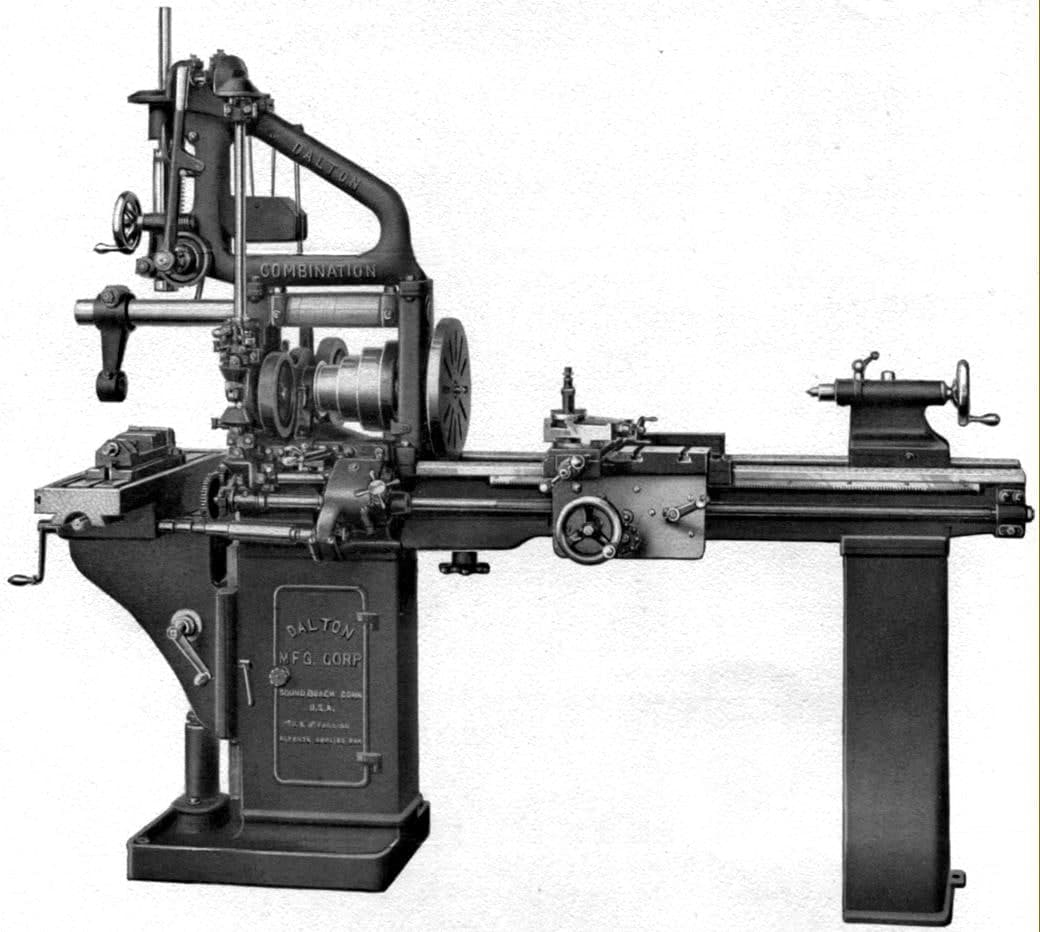
\includegraphics[width=0.7\textwidth]{ch-1/dalton}
	}
	\caption{Dalton Combinantion Machine}\label{fig:dalton}
\end{figure}

\paragraph{Piho Combination Machine}

Piho Combination Machine~(рисунок~\cref{fig:piho}) "--- комбинированный универсальный станок, производимый в конце 1940-х годов компанией Hartensteiner Maschinenfabrik, рекламировался производителем как устройство, которое будет использоваться в ремонтных мастерских. Существовало два типоразмера: б\'ольшая версия имела возможность регулирования высоты заднего центра от 175 до 300\:мм и межцентровое расстояние равное 1300 мм; меньшая (настольная версия) "--- от 60 до 100\:мм и 180\:мм между центрами соответственно. Обе модификации могли работать как токарный станок, а также как горизонтальный и вертикальный фрезерный станок.

Несмотря на компромиссы, заложенные в конструкции, в станке были реализованы составные направляющие скольжения, низкоскоростной узел заднего редуктора, ходовой винт, движущийся под станиной, а также был оснащен барабаном для реверса шпинделя и тонкой подачей с ременным приводом. Очевидно, что в качестве токарного станка он работал так же, как и любой другой обычный токарный станок даже меньшего типоразмера. Однако наличие дополнительного фрезерного модуля, позволяло ему приблизится по своим возможностям к современным обрабатывающим центрам. Более того, фрезерный модуль был оснащен пинолью для быстрой подачей для сверления и имел возможность наклона в плоскости, перпендикулярной оси токарного станка. За счет большого размера расточного стола можно было ещё повысить универсальность станка, используя его в качестве горизонтального фрезерного.

\begin{figure}[ht]
	\centerfloat{
		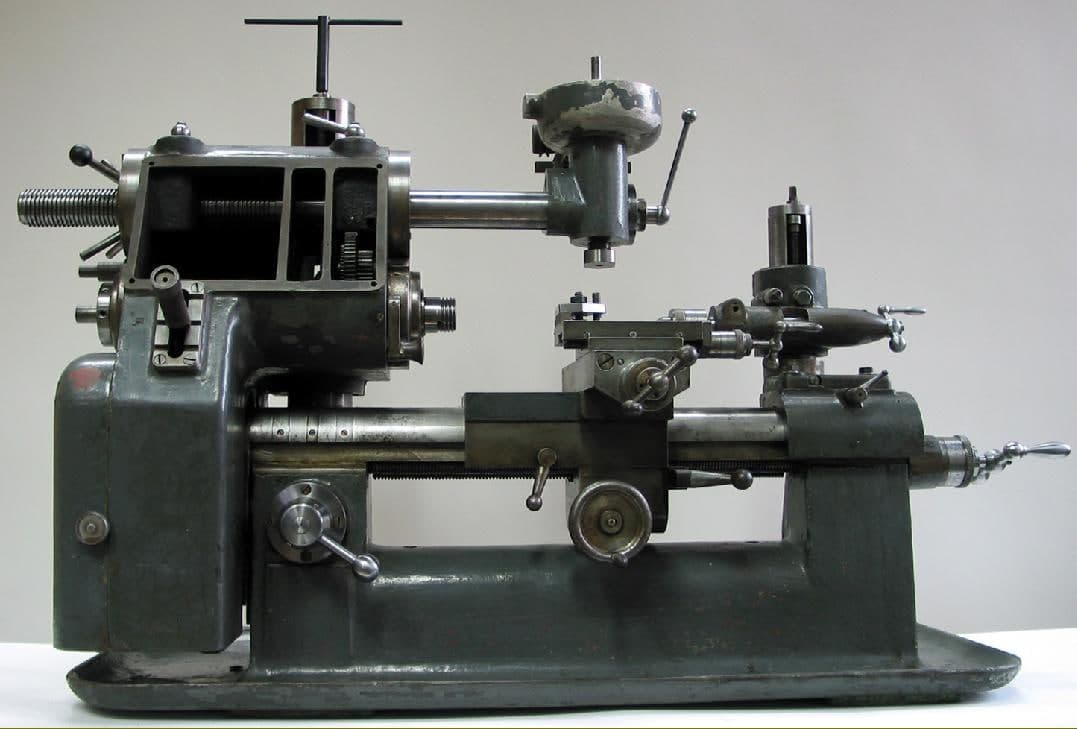
\includegraphics[width=0.7\textwidth]{ch-1/piho}
	}
	\caption{Piho Combination Machine}\label{fig:piho}
\end{figure}

\paragraph{Adcock \& Shipley Combination Machine Tool}

<<Универсал>> Adcock \& Shipley~(рисунок~\cref{fig:adcock-1}) обладал максимальной гибкостью и модульностью по сравнению с другими подобными станками. На площади всего 7 футов на 3 фута для б\'ольшей модели и 11 футов 6 дюймов на 3 фута 8 дюймов для меньшей помещались токарно-винторезный станок, круглошлифовальный станок для внутреннего и внешнего шлифования, вертикальный/горизонтальный фрезерный станок, а также сверлильный станок и специализированные модули для заточки инструмента. Вместо выдвижных или подъемных станин и передней бабки, которые использовались на многих других станках того же типа, Ryder был построен на основе обычного токарного станка, причем каждый отдельный модуль имел автономный привод и мог (кроме шлифовального станка) работать параллельно с другими модулями. Устройство было первоначально разработано для использования на борту корабля и соответствовало различным требованиям, установленным Британским адмиралтейством для этой цели. 

\begin{figure}[ht]
	\centerfloat{
		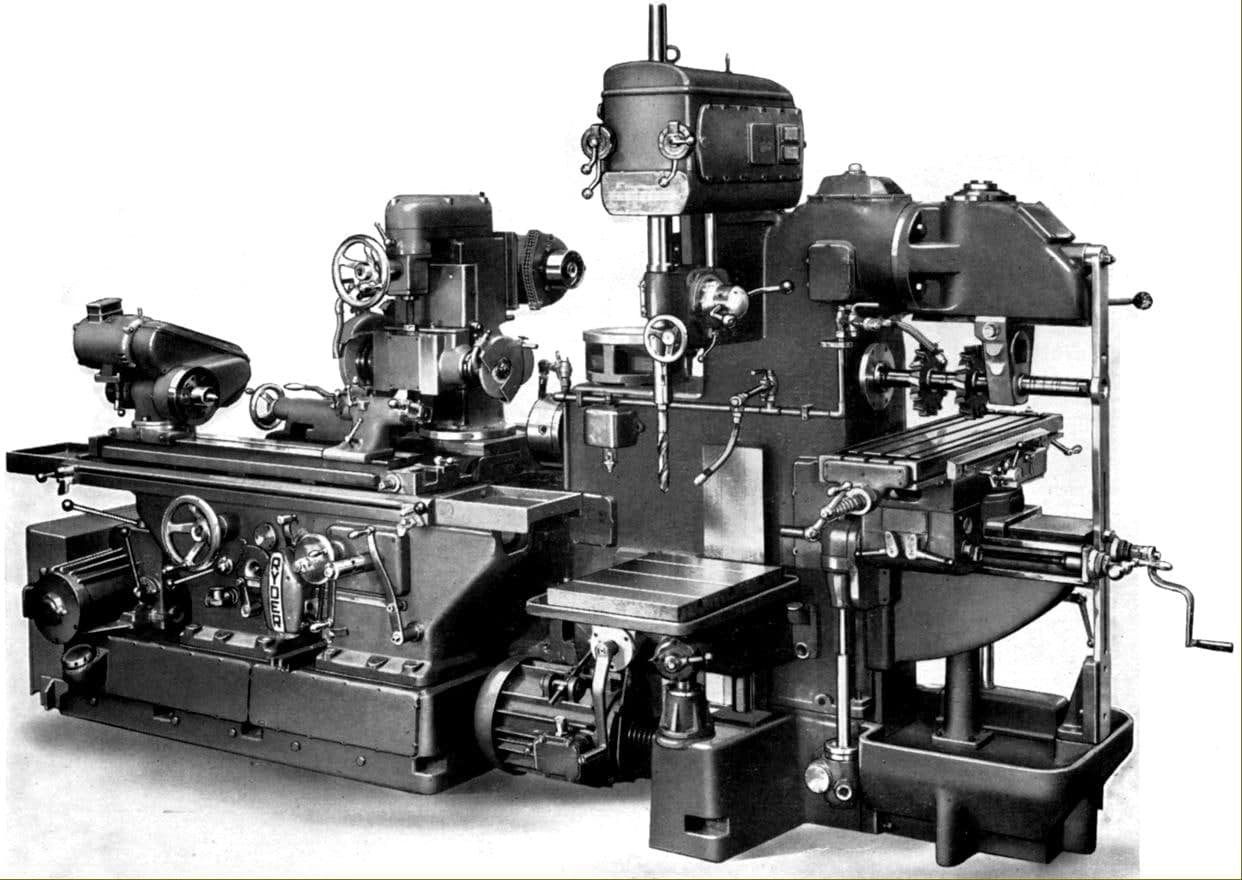
\includegraphics[width=0.7\textwidth]{ch-1/adcock-1}
	}
	\caption{Adcock \& Shipley Combination Machine Toolо, вид спереди}\label{fig:adcock-1}
\end{figure}

Токарный модуль обладал следующими характеристиками: высота над станиной 8 дюймов, расстояние между центрами 18 дюймов, коробка передач из 8 скоростей, обеспечивающая максимальную частоту вращения шпинделя в 1020 об/мин., трехфазный привод на 3 л.с., 1760 об/мин. Проходное отверстие шпинделя было всего 0,75 дюйма, что вряд ли соответствовало той работе, для выполнения которой мог бы потребоваться рассматриваемый станок. Также на станке был установлен упрощенный редуктор для нарезания резьбы с ходовым винтом, позволявшим нарезать дюймовые резьбы с шагом от 4 до 100 ниток на дюйм. Для автоподачи суппорта использовался отдельный ходовой вал, а ходовой винт был нужен исключительно для нарезания резьб.

Фрезерный модуль обладал оригинальной конструкцией с горизонтальным и вертикальным шпинделями. Рабочая поверхность фрезерного стола была размером 26 на 6 дюймов с продольным ходом 10 дюймов и поперечным всего 5,5 дюйма, вертикальный ход стола составлял 10 дюймов, что было крайне мало по сравнению со схожими по размерам универсальными фрезерными станками того времени. Оба шпиндели были рассчитаны на инструмент под конус ISO 40, горизонтальный мог вращаться с частотой от 48 до 970 об/мин, вертикальный "--- от 77 до 1575 об/мин.

Универсальный стол шлифовального станка с возможностью поворота на 45 градусов по часовой стрелке и 15 градусов против часовой стрелки был установлен параллельно станине токарного станка и использовался как опора для шлифовальной головки. Два зубчатых колеса соединяли головку с органами управления в передней части станка. Максимальная высота заготовки над столом составлял 7 дюймов, максимальная длина "--- 10 дюймов. Также была возможна заточка различного режущего инструмента. Подача охлаждающей жидкости к шлифовальной головке представляла собой отдельный блок, разработанный, чтобы избежать загрязнения другой охлаждающей жидкости (подаваемой на токарный, фрезерный и сверлильный модули) абразивными частицами.

Сверлильный модуль устанавливался на задней части <<шпиндельной бабки>> токарного станка и имел шесть скоростей от 420 до 5000 об/мин с мощностью, обеспечиваемой отдельным двигателем мощностью 0,5 л.\,с. Диапазон выбора инструмента был обусловлен использованием в патроне конуса Морзе 1, что ограничивало применение данного модуля для легких работ~(рисунок~\cref{fig:adcock-2}).

\begin{figure}[ht]
	\centerfloat{
		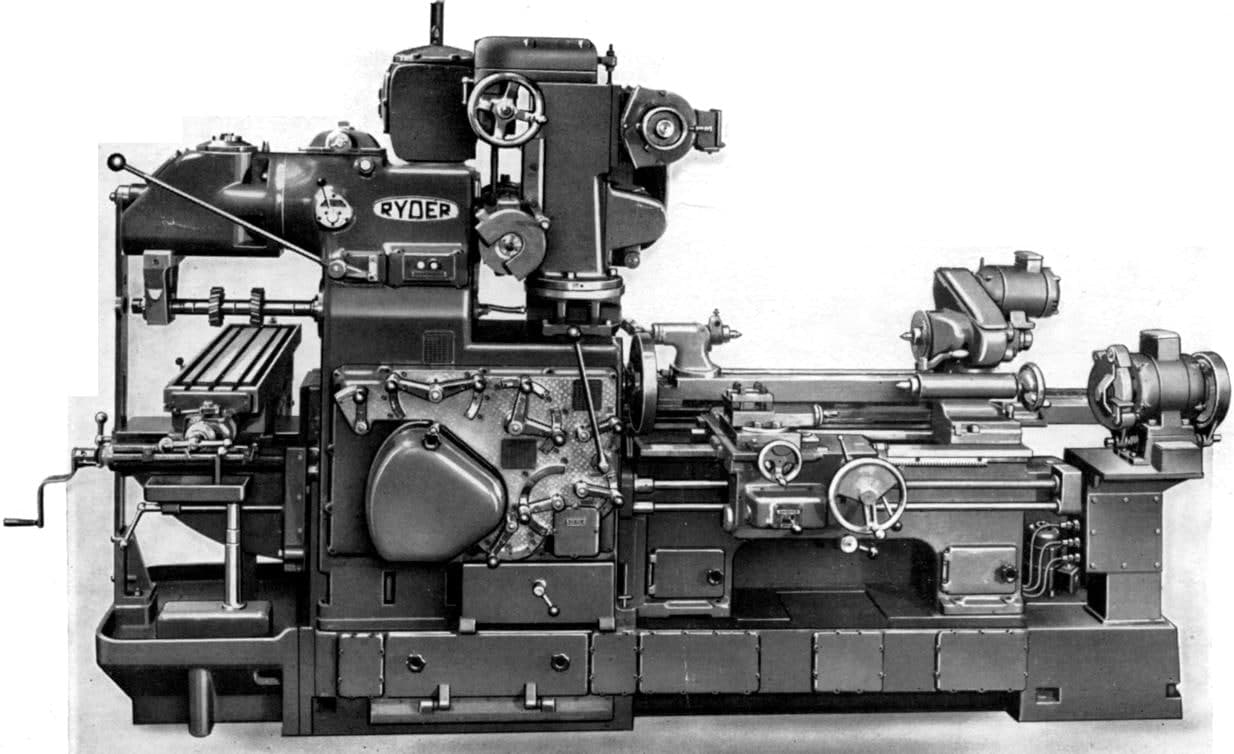
\includegraphics[width=0.7\textwidth]{ch-1/adcock-2}
	}
	\caption{Adcock \& Shipley Combination Machine Tool, вид сзади}\label{fig:adcock-2}
\end{figure}

\subsection{Агрегатные станки}

Агрегатными станками (АС) называется оборудование, которое состоит из стандартизованных и специальных агрегатов, сборочных узлов и деталей~(рисунок~\cref{fig:agr-example}). Доля специально изготовленных узлом при этом меньше доли стандартизованных и нормализованных узлов. Конфигурация агрегатных станков происходит за счёт объединения всех его узлов в единый агрегат (станок, рабочий комплекс). Для данного агрегата всегда используется \textit{общая (монолитная)} системой управления и контроля. АС в подавляющем большинстве случаев применяют в \textit{крупносерийном и массовом производстве}. Первые агрегатные станки управлялись по аналогии со станками-автоматами, повсеместно распространенными в 60--70х годах, затем появились станки с ЧПУ. Это дало возможность использовать агрегатные станки уже и в серийном производстве. Все современные агрегатные станки управляются с помощью ЧПУ, однако в единичном и малосерийном производстве данный тип оборудования не использовался никогда. На агрегатных станках возможно осуществлять многоинструментную и многопозиционную лезвийную и абразивную механическую обработку деталей. Ранние представители агрегатных станков могли выполнять только один вид обработки (главным образом этим видом обработки было сверление и резьбонарезание). Существующие на текущий момент модели могут комбинировать практически все технологические операции по механической обработке.

\begin{figure}[ht]
	\centerfloat{
		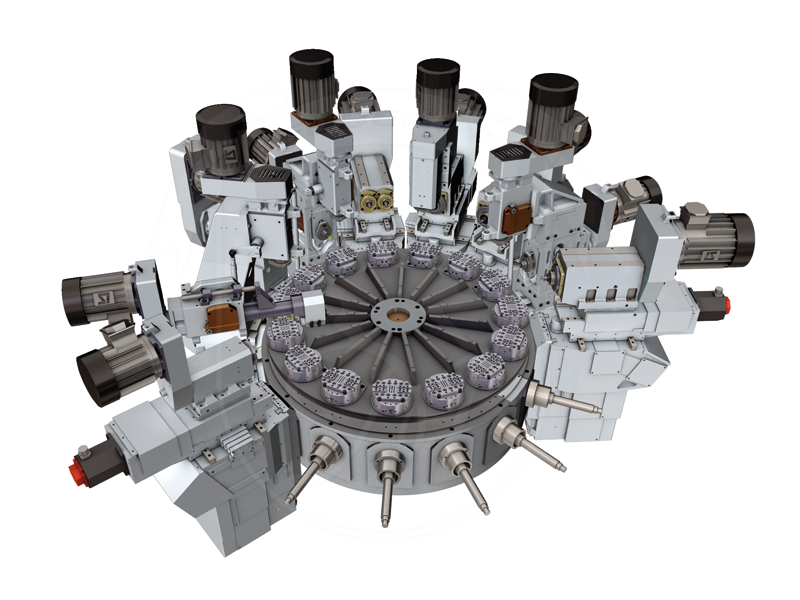
\includegraphics[width=\textwidth]{ch-1/agr-example}
	}
	\caption{Пример агрегатного станка}\label{fig:agr-example}
\end{figure}

Термин <<агрегатный станок>> впервые был использован и применялся в СССР. Однако существовали и существуют зарубежные станочные системы по сути своей являющиеся агрегатными станками. В литературе подобные станки именуются <<реконфигурируемыми производственными системами>>\footnote{От англ. \textit{Reconfigurable Machine Tools}.} или сокращенно RMS~\cite{lee1997reconfigurability, mehrabi2000}. RMS "--- это достаточно широкий класс промышленного оборудования, лишь некоторые разновидности которого соответствуют характеристикам отечественных агрегатных станков.  Так, в патенте~\cite{US6349237} описывается производственная система (станок), имеющая изменяемую структуру. Данная система разработана на основе рыночного спроса и может быть легко изменена для производства различных объёмов продукции одного семейства. Описанная система включает в себя множество рабочих станций с реконфигурируемыми агрегатами, подсистему числового программного управления, включающую множество реконфигурируемых контроллеров, а также реконфигурируемую систему обработки материалов. Также в патенте показано, что предлагаемое аппаратное обеспечение позволяет преобразовывать станки, например, путем перемещения их шпиндельных узлов. Производственные мощности рассматриваемой системы быстро адаптируются к рыночным колебаниям спроса на продукцию. Функциональность легко адаптируется к производству новых продуктов того же семейства. Подобные станки облада.т определенными ключевыми характеристиками (например, модульностью, интегрируемостью, настройкой, конвертируемостью и диагностируемостью), которые необходимы для быстрой и рентабельной реконфигурации. Также в патенте предоставляется методика разработки таких станков и дополнительная методика для изменения производственной мощности, включая реконфигурацию и наращивание парка подобных станков. 

Существуют и другие подобные станочные системы, поэтому в рамках данного обзора под термином <<агрегатный станок>> будут, в частности, подразумеваться и зарубежные системы класса RMS. Как и любое другое оборудование приборостроительного производства, агрегатные станки делятся на специальными и специализированными. Очевидно, что специальные предназначены для обработки одной или несколько деталей одновременно, в свою очередь, специализированные агрегатные станки нацелены на последовательное формообразование нескольких деталей, требующего незначительного изменение конфигурации АС. В зависимости от потребностей производства АС могут работать как автономно, так и в составе гибких производственных систем.

Принцип агрегатирования АС базируется на том положении, что вместо проектирования всех узлов при создании нового станка используют ранее использованные узлы. Из данных узлов получается определенная компоновка, которая и становится новым станком. Для осуществления данного процесса заранее разрабатывается ряд однотипных узлов (агрегатов) разных типоразмеров и мощности приводов (если узел или агрегат включает в себя отдельную силовую часть). Узлы и агрегаты, входящие в этот ряд называются нормализованными или унифицированными. Нормализованные узлы дают возможность спроектировать АС, практически полностью удовлетворяющий используемому технологическому процессу обработки той или иной заготовки. Агрегатные специальные станки обладают рядом существенных преимуществ преимущества перед другими станками, применяемыми в массовом и крупносерийном производстве:

\begin{itemize}
	\item АС позволяют создавать станки специально под конкретный технологический процесс. То есть в случае применения АС у технологов появляется возможность сначала разработать телеологический процесс, а потом сконфигурировать под него АС из уже готовых и отлаженных узлов и агрегатов. При этом нет необходимости оптимизировать или изменять технологический процесс под конкретные производственные возможности.
	\item АС позволяют осуществлять многоинструментную обработку заготовок, что дает возможность существенно повысить производительность производства.
	\item АС дают возможность выполнения разнообразных технологических операций на одном и том же станке путем простое его переналадки.
	\item Использование АС позволяет постоянно и непрерывно улучшать оборудование, используемое на производстве. Появляется возможность модернизироват не весь станок целиком, а лишь тот узел (агрегат), который морально или физически и требует замены.. То же самое касается и ремонтопригодности, сломавшийся узел может быть быстро заменен на такой же работоспособный (находящий в резерве), а после ремонта основного первоначального узла, он будет возвращен на склад хранения, для резерва на случай будущих поломок.
	\item При использовании АС увеличивается надежность\footnote{Здесь под надежностью понимается способность оборудования сохранять в течение продолжительного промежутка времени значения своих основных параметров в заданных интервалах.} работы оборудования, созданного из проверенных и отлаженных нормализованных узлов;
	\item В случае необходимости создания специального оборудования, оно также собирается из серийных узлов, что в целом удешевляет его.
\end{itemize}

Тем не менее, помимо плюсов, АС обладают и рядом недостатков, которые в настоящее время сильно сократили спрос на эти станки даже для \textit{массового производства}:

\begin{itemize}
	\item Для всех деталей, даже совсем незначильно отличающейся от уже существующей, необходимо делать (конфигурировать) новый специальный станок.
	\item АС в силу своей универсальности имеют более высокую стоимость, поэтому экономически могут оправдать себя только в условиях реального массового производства.
\end{itemize}


В процессе развития АС предпринимались многочисленные попытки устранить эти недостатки, в частности, было установлено, что специальное станочное оборудование должно удовлетворять трем основным условиям:

\begin{itemize}
\item позволял производить быструю переналадку и изменение конфигурации для обработки различных типов деталей при сохранении достаточно высокой производительности получаемого оборудования (это самое главное, поскольку стоимость основных средств составляет значительную долю в себестоимости продукции);
\item позволил в кратчайшие сроки спроектировать и изготовить новые виды оборудования;
\item имел невысокую стоимость, что подразумевает довольно быструю окупаемость.
\end{itemize} 


Стоит отметить, что по большей части АС для \textit{отдельных производственных условий} могут удовлетворять всем этим требованиям. Рассмотрим более подробно принцип унификации, который применяется в АС, в дальнейшем это будет полезно для понимания отличий методики унификации АС и рассматриваемого в данной работе модульного технологического оборудования. Унифицированными (иначе нормализованными) узлами АС называются узлы, конструкции которых проектируются с той целью, чтобы быть основой для любого станка, который будет проектироваться на их основе. Из этого несложно сделать вывод о том, унифицированные узлы могут применяться в станках самых разных конфигураций. К нормализованных узлам АС относятся~(рисунок~\cref{fig:agr-machine}):

\begin{itemize}
	\item боковые станины;
	\item станины;
	\item поворотные делительные столы;
	\item силовые бабки;
	\item отдельно стоящие блоки крепления (cтойки); 
	\item проставочные плиты.
\end{itemize}

\begin{figure}[ht]
	\centerfloat{
		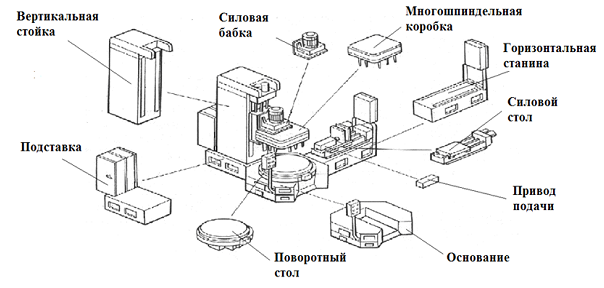
\includegraphics[width=\textwidth]{ch-1/agr-machine}
	}
	\caption{Структура узлов агрегатного станка}\label{fig:agr-machine}
\end{figure}

В случае многошпиндельной обработки большого количества отверстий или при фрезеровании различных плоскостей заготовок корпусных изделий к силовым головкам дополнительно крепятся специальные сверлильные и фрезерные насадки. В случае необходимости создания специальных узлов их компонуют из нормализованных сборок и деталей. Конструкция подобных узлов определяется в соответствии с конструкции детали, которая подлежит обработки на АС. Отечественные реализации АС включали в себя несколько сотен наименований различных унифицированных узлов в более, чем 2500 исполнений и типоразмеров. Из подобных нормализованных агрегатов и сборочных единиц могло состоять до 75--80\% узлов АС.

Необходимо отметить, что основное назначение АС "--- механическая обработка сложнопрофильных изделий. Из этого следует, что общее количество силовых узлов, блоков, включающих в свой состав различные шпиндели, а также само расположение осей шпинделей обуславливается технологическим процессов, выполняемым на АС. Соответственно, по типу АС разделяются на~\footnote{Электронный ресурс: {\tiny\url{extxe.com/3563/agregatnye-stanki/}} (дата обращения: 15.10.2018).}: 

\begin{itemize}
	\item одноагрегатные;
	\item многоагрегатные;
	\item одношпиндельные;
	\item многошпиндельные;
	\item горизонтальные;
	\item вертикальные;
	\item наклонные;
	\item комбинированные;
	\item односторонние;
	\item многосторонние.
\end{itemize}

Очевидно,что однопозиционные АС в первую очередь рассчитаны на один неизменный установ заготовки. При этом обработка происходит с одной стороны, а положение заготовки в процессе обработки не изменяется. На многопозиционных станках, оснащенных поворотно-делительными столами механическая обработка заготовок может осуществляться в параллельном или последовательном режиме, но сразу в нескольких разных позициях относительно обрабатывающих инструментов.

Из всего вышесказанного можно сделать вывод о том, что основными нормализованными узлам АС являются так называемые силовые головки, определяющие технологическую операцию. В современных АС каждая силовая головка снабжена отдельным автономным электроприводом, поэтому могут сообщать какому-либо инструменту главное движение, либо осуществлять перемещение, например, делительного устройства. Для каждой силовой головки предусмотрен свой жестко запрограммированный цикл перемещения, включающий в себя подвод инструмента на ускоренной подаче, непосредственно рабочий ход инструмента (их может быть несколько в зависимости от технологического процесса), при необходимости может быть реализована выдержка в жёстком упоре и отвод инструмента на ускоренной подаче с последующем остановом. Как уже отмечалось ранее, первые образцы АС реализовывали данную циклограмму механически с помощью вращающегося кулачка, современные образцы АС реализуются ее исключительно посредством ЧПУ.

Параметры каждой силовой головки являются основанием для использования ее для конкретной технологической операции. К основным параметрами силовых головок относят:

\begin{itemize}
	\item мощность электропривода, обеспечивающего главное движение;
	\item наибольшее усилие, которое может быть приложено к заготовке при подаче;
	\item частота вращения приводного вала шпинделя обрабатывающей головки;
	\item пределы перемещения при линейной или круговой подаче;
	\item скорость холостого хода при перемещении заготовки относительно инструмента;
	\item скорость рабочего хода при перемещении заготовки относительно инструмента;
	\item длина рабочего хода при линейном перемещении;
	\item габаритные размеры блоков и головок.
\end{itemize}

Необходимо отметить, что силовые головки являются не единственными блоками АС. Для выполнения силовых операций: фрезерования с большим съёмом материала, растачивания, подрезки торцов большого диаметра требуются блоки большей жесткости. Для повышения жесткости силовых головок разработчики данной концепции пришли к следующему решению: в силовой головке разделили агрегаты, обеспечивающие главное движение и движение подачи. Таким образом, получилось два разных независимых узла: силовая бабка для реализации главного движения и отдельный силовой стол для обеспечения движения подачи.  

Помимо блоков, обеспечивающих прямолинейное движение заготовки по отношению к инструменту в АС часто использовались делительно-поворотные столы, основной задачей которых было закрепление специализированных приспособлений с заготовками. Данные столы обеспечивали поворот заготовки по отношению к инструменту на определенный угол. Также имелась возможность перемещать обрабатываемые заготовки из одного рабочего положения (установа) в другое. В этом случае заготовка была опять же была точно зафиксирована относительно режущего инструмента. 

Поворотные столы могли быть в вертикальном или горизонтальном исполнениях. Форма столов чаще всего была либо кольцевая, либо дискообразная. Такие столы перемещались только в горизонтальной плоскости. Если поворотный стол осуществлял вращение в вертикальной плоскости, то такой блок именовался <<барабан>>. При использовании барабанных блоков, приспособления с закрепленными в нем заготовками располагалось на периферийной поверхности барабана и заготовку можно было обрабатывать с двух сторон одновременно.

К современным станкам, которые могут быть отнесены к классу агрегатных, можно отнести Mikron MultiX\footnote{Электронный ресурс: {\small\url{https://www.mikron.com/machining-solutions/machining-systems/highly-productive-systems/multix/}} (дата обращения: 14.07.2018).}~(рисунок~\cref{fig:mikron}). Данное оборудование представляет собой платформу, являющейся основой для установки разнообразных станции обработки. Платформа выступает в качестве базового агрегата, а обрабатывающие станции являются сменными блоками. Существует три типоразмера базового агрегата, различающиеся количеством устанавливаемых на них блоков. Конфигурация платформы подбирается под конкретный технологический процесс.

\begin{figure}[ht]
	\centerfloat{
		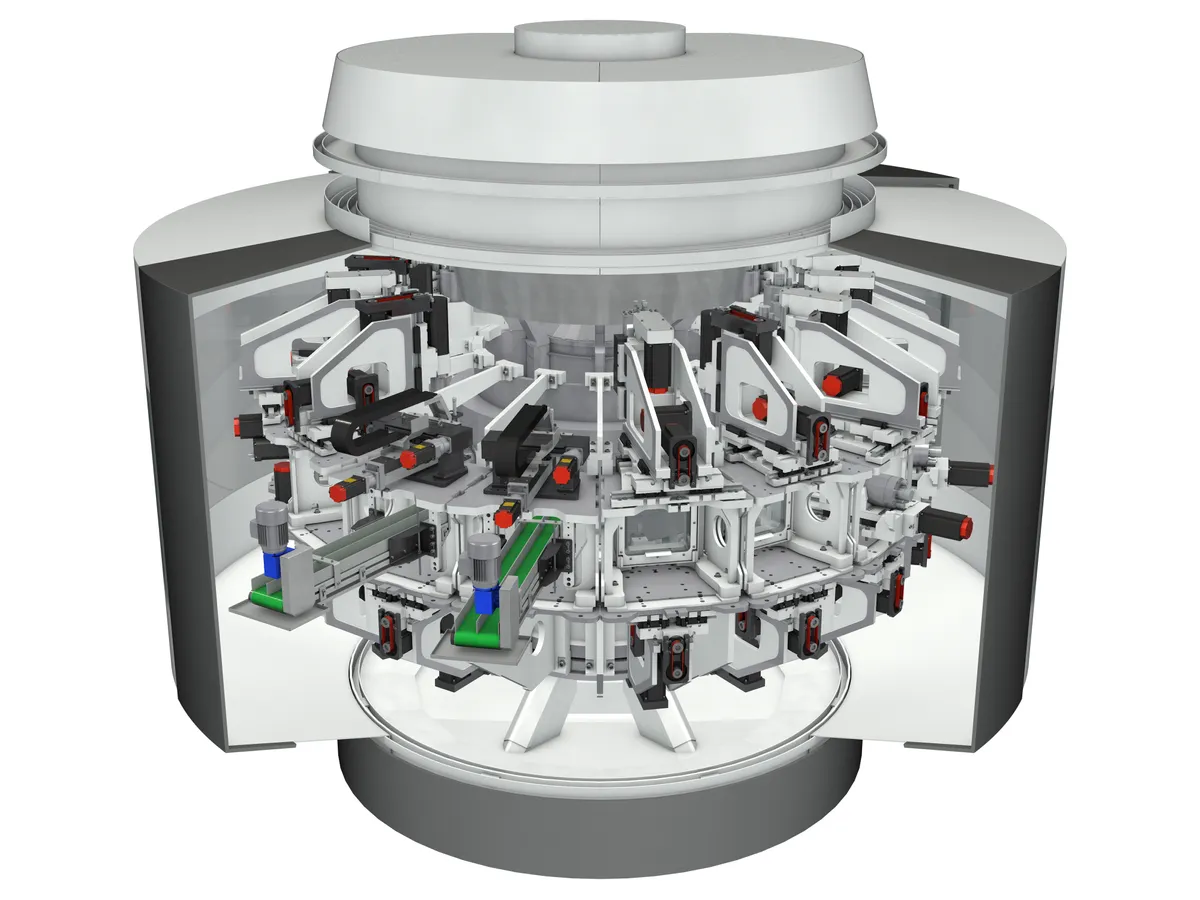
\includegraphics[width=0.7\textwidth]{ch-1/mikron}
	}
	\caption{Агрегатный станок Mikron MultiX}\label{fig:mikron}
\end{figure}

Таким образом, получается, что унификация и стандартизация АС сильно усложняется, т.\,к. конструкция не может быть разделена на равные по своим возможностям и габаритам блоки. По сути АС "--- это сложный унифицированный станок-автомат, где каждый блок имеет несколько разных исполнений, что в общем дает большое разнообразие полученного таким образом оборудования, но это оборудование нельзя считать модульным. Блоки АС неуниверсальны и могут выполнять свои функции только вместе с другими блоками, проектирование которых происходило одновременно. Агрегатные станки унифицированы только по присоединительным размерам и нет центрального блока, на который могли бы устанавливаться другие блоки, изменяя тем самым основную функцию оборудования. Также стоит еще раз повторить, что в основном АС применялись только для металлообработки и никогда не использовались для других видов обработки. На сегодняшний день в силу своей сложности и узкой направленности АС потеряли актуальность даже в рамках массового производства, однако сами базовые подходы, которые были положены в основу их функционирования могут и должны быть использованы для создания универсального модульного оборудования для условий мелкосерийного и единичного производства.

\section{Академические разработки в области модульного технологического оборудования} 

Наиболее полным отечественным исследованием, посвященном теме модульного оборудования является монография Олега Ивановича Аверьянова <<Модульный принцип построения станков с ЧПУ>>~\cite{averianov}. В работе дана комплексная оценка модульного принципа построения многоцелевых станков с ЧПУ, разработанная в московском экспериментальном научно-исследовательском институте металлорежущих станков. Автором проанализированы тенденции развития производства станков, актуальные на период конца 80-х годов, в том числе рассмотрены различные серийные и экспериментальные металлорежущие станки отечественного и зарубежного производства (к сожалению, подавляющее большинство указанно оборудования уже сняты с производства). Также указаны области рационального применения многоцелевых станков с использованием соответствующего математического аппарата. В данной работе теоретически описаны и алгоритмически подтверждены многие гипотезы, связанные с применением модульного оборудования именно в единичном и мелкосерийном производстве.  Однако на момент написания данной монографии основой промышленности были металлорежущие станки, поэтому другие виды обработки в рамках описанной модульной структуры автором не рассматривались. Более того, понятие <<информационные технологии>> в то время ещё не существовало, поэтому система ЧПУ в работе рассматривается как некоторый автомат по перемещению рабочих органов в пространстве (по аналогии со станками-автоматами механически управляемыми посредством кулачков). Естественно, возможность создания модульной децентрализованной автоконфигурируемой системы ЧПУ даже не рассматривается. В связи с распадом Советского Союза и отказом от плановой экономики, наработки, представленные в работе О.\,И Аверьянова. перестали быть актуальными, однако сама методическая основа построения модульного технологического оборудования могут и должны получить развитие в новых современных модульных системах.

Помимо О.\,И.~Аверьянова вопросами разработки модульного оборудования занимались такие отечественные исследователи, как В.\,Н.~Бетин~\cite{betin}, Л.\,П.~Бобрик~\cite{bobrik}, Л.\,С.~Брон~\cite{bron}, Д.\,А.~Куприянов~\cite{kuprianov}, В.~В.~Вяткина~\cite{minhat2009stepncmilluoa} и другие. 
	
Также существует достаточное количество зарубежных исследований, посвященных данной теме. Предпосылками к исследованиям в данной области стали многофункциональные универсальные металлорежущие станки, которые были описаны в разделе~\cref{sec:ch1/multifunc-machines}. Данное оборудование реализовывалось для решения конкретных технологических задач, при этом изначально какие-либо исследования самого принципа модульности не проводились. Модульная конструкция станка претерпевала постепенные изменения, модернизировалась и развивалась в различной степени с 1930-х годов. При этом менялась конструкция базового агрегата, система строительных блоков, применялся модульный дизайн, холонический дизайн, принципы реконфигурируемости конструкции и т.\,д. Концепция и метод модульного проектирования для структурной конфигурации приписываются Г.~Шлезингеру и Ф.~Кенигсбергеру. Первый предложил концепцию на примере конструкции передней бабки радиально-сверлильного станка, а второй применил этот метод к конструкции фрезерного станка марки Wanderer~[Spur, G., Produktionstechnik in Wandel, Carl Hanser Verlag, M{\"u}nchen/Wien, 1979]. Изначально термин <<модуль>> авторами не использовался, вместо этого подобный подход называли <<системой строительных блоков>>. Этот термин окончательно был заменен термином <<модульная конструкция>> самим профессором Кенигсбергером примерно в 1967\,г.

С этого момента и до сегодняшнего дня модульная конструкция в различной степени охватывала такие сферы зарубежных исследований, как проетирование производственных систем и станков, программного обеспечения и режущего инструмента. Сейчас происходит продвижение модульного принципа в некоторые новые области исследований промышленного производства. Например, в монографии Йошими Ито~\cite{ito2008modular} рассматривается модульный принцип конструирования металлорежущего оборудования с числовым программным управлением, представлены методы, позволяющие сократить время проектирования подобных модульных систем, повысить надежность их функционирования, снизить эксплуатационные затраты и упростить обслуживание и ремонт. В работе рассмотрены основы модульного проектирования технологического оборудования, методика определения характеристик модульных станков, описаны примеры применение модульных станков. Также рассматриваются принципы взаимодействия модулей в информационном плане и методика тестирования модульного оборудования.

Среди прочих работ можно выделить работу Светика~\cite{svetlik2020modularity}, посвященную модульному принципу построения производственных систем, в частности модульного технологического оборудования. Предложена концепция модульной технологической системы, разработана математическая модуль функционирования и сборки подобных систем, определены основные их параметры. Рассмотрены примеры предложенной концепции в приложении к различным видам технологического оборудования: промышленным роботам, обрабатывающим центрам и логистическим системам.

В работах Бортолини~\cite{bortolini2019reconfigurability, bortolini2019dynamic} приведен пример применения модульного подхода в ячеистом производстве~(сокр.~\textit{ЯП}). Показано, что обычно в ЯП каждая ячейка используется для определенного семейства деталей, что сокращает объём использованного материала, время погрузочно-разгрузочных операций, а также объём незавершенного производства. Предлагается модифицировать имеющееся ЯП посредством внедрения модульного подхода. Автором предложена оригинальная модель оптимизации, основанная на теории линейного программирования, для разработки альтернативной маршрутизации деталей. В данной модели ЯП строиться из реконфигурируемого оборудования, состоящего из множества основных и вспомогательных модулей. При использовании различных вспомогательных модулей на одной и той же единице реконфигурируемого оборудования становятся доступными различные операции. В предлагаемом подходе происходит оптимизация набора модулей и маршрутизация движения объектов производства между ячеками ЯП. Проведен сравнительный анализ, в которой сопоставляется предложенная и традиционная модели ЯП. Анализ показывает, что предложенная модель позволяет уменьшить время на перемещение объектов производства между ячейками на 58,6\%, а общее снижение времени примерно на 53,3\%.

Ли в работе~\cite{li2020modular} была описана информационная модель модульного проектирования станков с ЧПУ на основе  потребительского спроса, путём анализа требований клиентов. На основе предложенной функции качества получается базовая структура станков, а в результате анализа нечеткой кластеризации получается уточненное функциональное разделение на модули и формируется диаграмма динамической кластеризации. На основе метода предпочтения порядка по подобию оценивается окончательная схема разделения модулей станков. Данный подход декомпозиции оборудования на отдельные блоки апробирован на примере горизонтально-фрезерных станков с ЧПУ компании Shenyang Machine Tool Group. Анализ предложенной конструкциии показывает, что система модульного разделения является эффективной для данного типа оборудования. Подобный подход описан в работе Шень~\cite{sheng2017lifecycle}, только в качестве метрики оценки эффективности получаемой модульной конструкции здесь используются параметры жизненного цикла изделия.  

\section{Модульные системы управления технологическим оборудованием}\label{sec:ch1/sec2}
%Добавить сюда про смузи и LinuxCNC

Анализируя эволюцию современной индустрии, можно сделать вывод о том, что наиболее многообещающим направлением развития является создание гибких распределенных автоматизированных производственных линий. Новая концепция массового производства была создана в результате Четвертой промышленной революции (или Индустрии 4.0) и постепенного распространения индустриальных кибер-физических систем. Подходы, применяющие жесткую последовательную логику реализации этапов технологического процесса в крупносерийном и массовом производстве постепенно преобразуются для условий мелкосерийного производства на заказ. Как уже отмечалось ранее, продолжается развитие малых инновационных предприятий. В итоге меняется подход к проектированию современного интеллектуального оборудования.

Первые станки с числовым программным управлением появились в середине XX~века. Основной областью применения такого оборудования изначально было массовое производство. Первые системы числового программного управления были сложными и дорогими. Для внедрения таких систем в существующее производство требовался длительный период пуско-налодочных работ и обкатки на конкретном технологическом процессе. Станки с ЧПУ крайне плохо поддаются модернизации, поэтому период их эксплуатации является достаточно длительным и может достигать нескольких десятилетий.

Данные обстоятельства сильно мешают при внедрении современных информационный технологий в промышленность. Это обуславливается тем, что даже незначительное изменение структуры производства требует полного изменения производственного цикла, либо, как минимум, создания вспомогательных уровней управления на уровне цехов и участков.В противном случае невозможно грамотно интегрировать старое оборудование с современной кибер-физической системой. Однако данный этап неизбежен при постепенном смене парка технологического оборудования и перехода к новым подходам в производстве.
Следовательно, необходимо переосмыслить саму парадигму проектирования оборудования с ЧПУ, и возможность подключения нового оборудования к информационной среде связи по открытому протоколу становится весьма важной.

Современными исследователями были предприняты попытки реализации подобного подхода. Например, Григорьев и Мартынов в своих исследованиях предлагают подход к разработке гибкого ядра ЧПУ на основе программной платформы, реализованной в виде автономных библиотечных модулей. Открытая архитектура этой системы включает в себя различные абстрактные уровни, относящиеся к различным человеко-машинным интерфейсам, и возможность описания компонентов системы на разных языках программирования. Подключение компонентов системы осуществляется через шину Fieldbus~\cite{Grigoriev2014517}.

Бин и др. описывают открытую платформу для создания систем ЧПУ, эта система состоит из набора многоцелевых компонентов, которые могут использоваться многократно, и набора коммуникационных модулей для их соединения~\cite {Bin200473}. Похожий подход представлен в статье Ма~\cite{MA2007272}.
Моралес-Веласкес и др. предложена система (платформа) ЧПУ с открытой архитектурой на основе многоагентной системы программных и аппаратных компонентов под названием MADCON. Аппаратные блоки предлагаемой ими системы объединяют функции управления и мониторинга, обеспечивая открытую архитектуру на основе ПЛИС для реконфигурируемых приложений. Программные компоненты используют структуру XML для файлов описания системы, объединяя такие функции, как язык описания блок-схем и графический пользовательский интерфейс~\cite{MoralesVelazquez2010407}.

Работы Вербы~\cite{Verba2016} и Празереса~\cite{Prazeres7471301} посвящены концепции <<Туман вещей>>.\footnote{Сокр. от англ. \textit{Fog of Things}.} Эта концепция представляет собой современную интерпретацию Интернета вещей\footnote{От англ. \textit{Internet of Things}.}, который, по сути, является основой многих индустриальных кибер-физических систем. Туман вещей позволяет создать более однородную информационную среду связи, тем самым улучшая и упрощая протокол связи компонентов.

В работе Хана~\cite{han2007development} рассматривается контроллер с открытой архитектурой, который может быть основой для различного оборудования с ЧПУ. Разрабатываемый контроллер имеет модульную архитектуру, а в качестве аппаратной  платформы использует персональный компьютер. Основная цель работы "--- разработать методику построения программно-аппаратная платформа системы ЧПУ. Также исследуются методы статического моделирования контроллера с открытой архитектурой, включающие технологию объектно-ориентированного программирования, технологию применения динамических библиотеки и разделения  системных модулей. Авторы обсуждают динамическое моделирование поведения  и представление потока данных контроллера с открытой архитектурой, которые  описаны с помощью иерархической модели конечного автомата. Для разработки  библиотеки программных функциональных компонентов авторы создали модель  многократно используемого программного модуля. В качестве испытательного  стенд выступает трёхосевой фрезерный станок. Для данного станка был успешно  разработан программный код системы ЧПУ, основанной на описанной библиотеке функциональных модулей с применением методики конфигурирования  системы. Результаты экспериментов показывали, что, помимо увеличения степени повторного использования программного кода и открытости, применение  вышеупомянутой методологии приводит к значительному сокращению времени  разработки, а также стоимости обслуживания конечного оборудования с ЧПУ.

\section{Промышленные аналоги предлагаемой модульной платформы}\label{sec:ch1/industrial-examples}
%Добавить сюда из материалов


В настоящем разделе будут рассмотрены проекты и готовые продукты, которые обладают свойством модульности и возможности переналадки. Первый критерий по, которому проходило сравнение "--- \textit{универсальности рабочего органа}, то есть возможность путём простой переналадки менять тип оборудования. 

На сегодняшний день на рынке представлены несколько типов универсальных модульных настольных станков нижнего ценового диапазона. Одним из наиболее известных производителей подобного оборудования является компания \textit{Proxxon}~(рисунок~\cref{fig:proxxon}), выпускающая различные настольные станки <<хоббийного>> класса, в основном токарно-фрезерно-сверлильной группы, распиловочное оборудование и ручной электроинструмент. Большое количество универсальной оснастки и~взаимозаменяемость многих частей оборудования Proxxon позволяет использовать его в небольших мастерских, а также на малых инновационных предприятиях, но с рядом ограничений:

\begin{itemize}
	\item В базовой комплектации все оборудование ручное. Возможность переделки под числовое программное управление является опцией. Возможности ЧПУ сильно ограничены.
	\item Спецификации оборудования закрыты, создание своих модулей невозможно, либо возможно, но только с~применением реверс-инжиниринга.
	\item Все оборудование Proxxon субстрактивного типа, возможность использовать его для создания 3d-принтера или контрольно-измерительной машины отсутствуют, так как нет единой модульной структуры блока управления ЧПУ, а также фирменного программного обеспечения.	
\end{itemize}

\begin{figure}[ht]
	\centerfloat{
		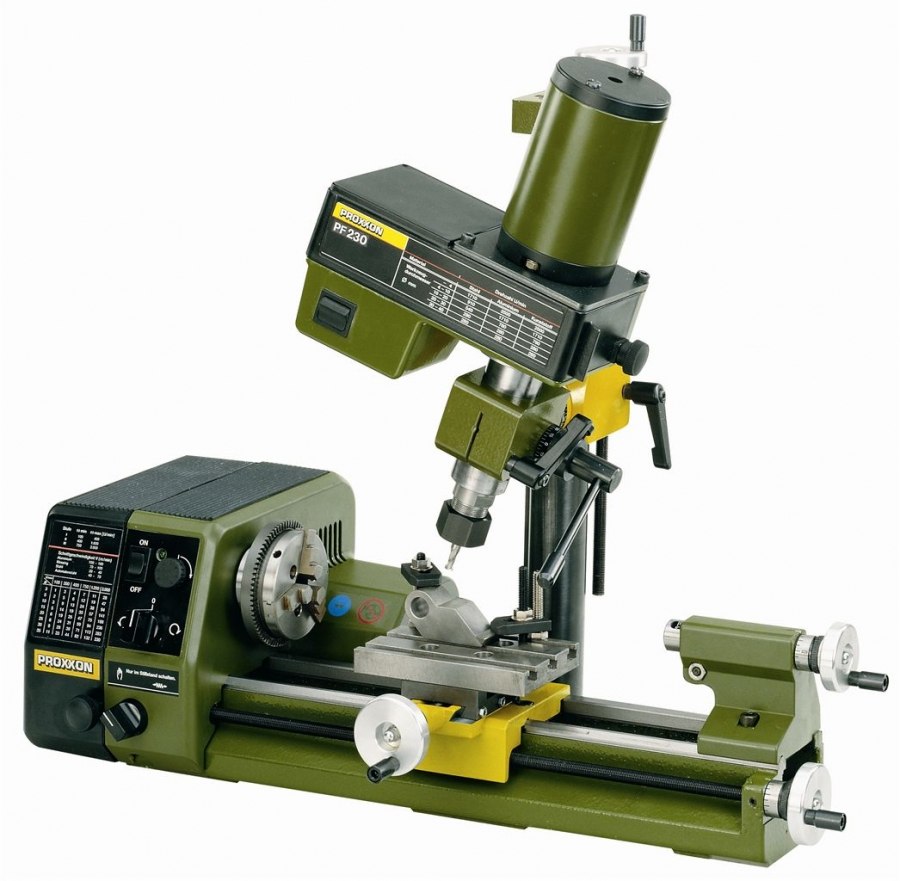
\includegraphics[scale=0.27]{ch-2/image1.png}
	}
	\caption{Пример оборудования компании Proxxon}\label{fig:proxxon}
\end{figure}

Стоит также отметить настольные модульные универсальные станки, выпускаемый немецкой компанией TheCoolTool\footnote{Электронный ресурс: {\small\url{thecooltool.com}} (дата обращения: 07.05.2020).}, в~особенности модели UNIMAT~1~(рисунок~\cref{fig:unimat-2}) и UNIMAT CNC~(рисунок~\cref{fig:unimat-2}).

\begin{figure}[ht]
	\centerfloat{
		\hfill
		\subcaptionbox{\label{fig:unimat-1}}{%
			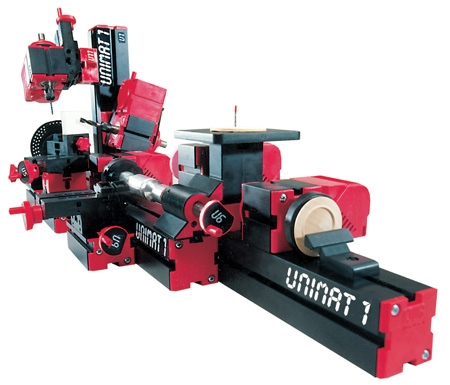
\includegraphics[width=0.4\linewidth]{ch-2/image2}}
		\hfill
		\subcaptionbox{\label{fig:unimat-2}}{%
			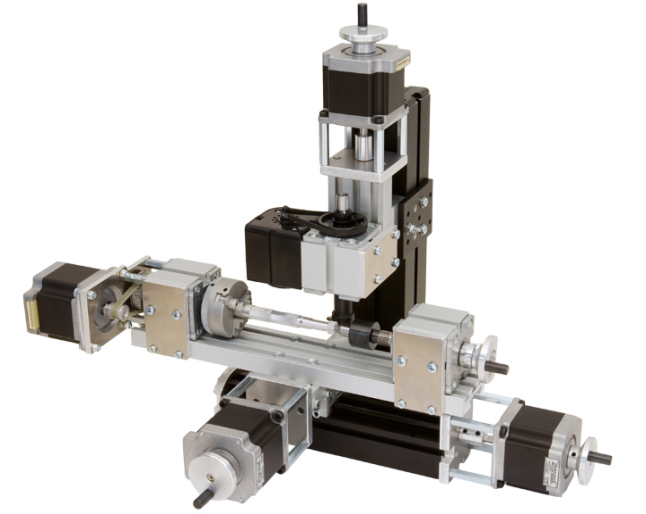
\includegraphics[width=0.4\linewidth]{ch-2/image3}}
		\hfill
	}
	\caption[Настольные модульные станки UNIMAT 1 и UNIMAT CNC]{Настольные модульные станки UNIMAT 1 (\textit{а}) и UNIMAT CNC (б)}\label{fig:unimat}
\end{figure}

Первый из рассматриваемых станков представляет собой модульную систему <<6 в 1>> с ручным управлением (переделка под ЧПУ возможна только с применением специальных доработок и реверс-инжиниринга), то есть позволяет в зависимости от компоновки модулей производить:

\begin{itemize}
	\item Распиловку деревянных и металлических заготовок вертикально расположенным ножовочным полотном.
	\item Токарную обработку деревянных заготовок.
	\item Токарную обработку металлических заготовок.
	\item Плоское торцевое шлифование с возможностью снятия шлифовального блока для ручной обработки шлифовальным кругом.
	\item Вертикальное и горизонтальное фрезерование.
	\item Сверление с возможностью поворота сверлильной головки на 360$^{\circ}$ или снятия её для ручного сверления.
\end{itemize}

Возможность совмещения двух операций без переналадки оборудования отсутствует.

Второй является токарно-фрезерно-сверлильным модульным станком с ЧПУ, в котором в зависимости от компоновки существует возможность управления шестью осями одновременно, что позволяет совмещать операции обработки без перенастройки модулей. Достоинством данного оборудования является большая открытость программной архитектуры, что подтверждается возможностью использовать для управления осями станка не только фирменное закрытое программное обеспечения, но и открытое решение EMC2, построенное на базе свободной операционной системы Linux. При этом сам станок представляет собой лишь набор управляемых электроприводов без внутреннего блока управления, что требует постоянного подключения к персональному компьютеру, приобретаемому отдельно.

К недостаткам можно отнести:

\begin{itemize}
	\item закрытую аппаратную архитектуру рассматриваемого продукта, что существенно усложнит переделку данного решение подо что-то отличное от металлообрабатывающих станков;
	\item неудачную геометрическую компоновку станка, что также ставит по сомнение возможность его переделки под другие нужды (например, очевидно, что подобная кинематическая схема вряд ли позволит использовать ее в качестве трёхмерного принтера или контрольно-измерительной машины);
	\item отсутствие портала, что влечет за собой снижение жёсткости связки координатных осей, а, следовательно, и жёсткости станка в целом. Последнее будет особенно заметно при максимально удалении осей, из-за чего может пострадать точность обработки. Данное предположение подтверждается спецификациями, размещенными на сайте производителя, где указывается, что точность установки не может превысить 80\,мкм.
	\item низкую мощность приводов осей, а также очень небольшие рабочие ходы по некоторым из них.
\end{itemize}

Получается, что за исключением возможности использования свободного программного обеспечения рассматриваемый продукт не является полностью модульном, это переналаживаемый станок с расширенными возможностями ЧПУ.

Второй параметр, по которому проводилось сравнение с существующими аналогами "--- \textit{открытая аппаратная архитектура}, позволяющая создавать новые типы оборудования без необходимости создания каких-то дополнительных переходных блоков и применения реверс-инжиниринга.

Для сравнения были рассмотрены два проекта, целью которых является создание открытой платформы универсального оборудования с ЧПУ:

\begin{enumerate}
	\item Build Your Own CNC.\footnote{Электронный ресурс: {\small\url{buildyourcnc.com/cnckit2.aspx}} (дата обращения: 31.12.2019).}
	\item Shapeoko.\footnote{Электронный ресурс: {\small\url{shapeoko.com}} (дата обращения: 31.12.2019).}
\end{enumerate}

Рассмотрим оба этих проекта более подробно. \textit{Build Your Own CNC}~(рисунок~\cref{fig:byocnc}) "--- коммерческий проект по созданию универсального сборного оборудования с числовым программным управлением. Может считаться условно открытым, так как на сайте производителя отсутствуют чертежи и прочая техническая документация, необходимая для самостоятельного изготовления того или модуля оборудования (за исключением файлов раскроя основных корпусных деталей), но при этом компания принимает запросы от пользователей на создание новых модулей (новых типов оборудования). Финансирование данных исследований проводится за счёт средств, полученных в качестве пожертвований от пользователей, а также за счёт основного бизнеса компании "--- производства и продажи модулей и готовых сборных устройств.

На сегодняшний день в рамках проекта \textit{Build Your Own CNC} реализовано достаточно большое количество модулей и готовых устройств, среди которых можно выделить:

\begin{itemize}
	\item Установку для лазерной резки и гравирования.
	\item Трёхкоординатное фрезерные и сверлильные станки различных компоновок и типоразмеров со множеством сменных головок, среди которых необходимо выделить печатающую головку, позволяющую создать на основе предлагаемой платформы 3d-принтер типа FDM\footnote{Сокр.~от~англ. \textit{Fused Deposition Modeling} "--- моделирование методом наплавления.}.
	\item Распиловочные вертикальные станки.
	\item Установку для автоматического размещения электронных компонентов на печатной плате\footnote{Англ. \textit{Pick and Place machine}.}
\end{itemize}

\begin{figure}[ht]
	\centerfloat{
		\hfill
		\subcaptionbox{\label{fig:byocnc-1}}{%
			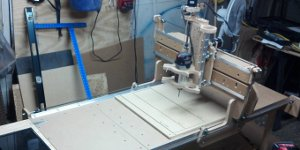
\includegraphics[width=0.5\linewidth]{ch-2/image4}}
		\hfill
		\subcaptionbox{\label{fig:byocnc-2}}{%
			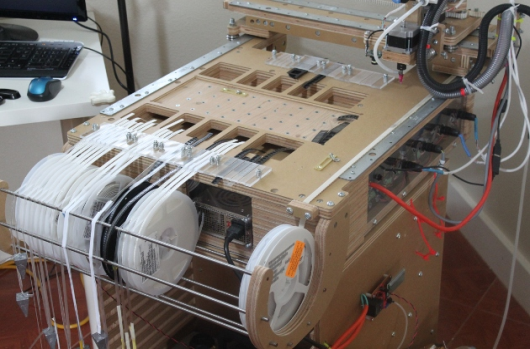
\includegraphics[width=0.5\linewidth]{ch-2/image5}}
		\hfill
	}
	\caption[Примеры оборудования, созданного в рамках проекта \textit{Build Your Own CNC}]%
	{Примеры оборудования, созданного в рамках проекта \textit{Build Your Own CNC}: фрезерный станок портального типа (\textit{а}), установка для позиционирования электронных компонентов на печатной плате (\textit{б})}\label{fig:byocnc}
\end{figure}

В планах компании также разработать:

\begin{itemize}
	\item Пятикоординатный фрезерный станок.	
	\item 3d-принтер, использующий технологию фотолитографии.
	\item 3d-принтер, использующий технологию селективного лазерного спекания.
	\item Станки токарной группы.
	\item 3d-сканер.
\end{itemize}

К недостаткам данного проекта можно отнести следующие:

\begin{itemize}
	\item Как уже отмечалось ранее, проект не является полностью открытым с точки зрения аппаратного обеспечения.
	\item На текущий момент реализовано очень малое количество типов оборудования. Отчасти это связано с первым недостатком, так как спецификации закрыты и разработкой новых модулей и типов оборудования занимаются только сотрудники компании.
	\item Отсутствует единая универсальная кинематическая схема, из-за чего для каждого нового вида оборудования необходимо проектирование новой кинематической схемы, а также сопутствующие этому процессу расчеты и моделирование.
	\item Отсутствует единый подход к проектированию линейных приводов. Предполагается возможность использования как ходовых винтов с трапециевидной резьбой, так и передач на основе зубчатых ремней и цепей. Особо настораживает использование цепных передач в прецизионных настольных станках для установки электронных компонентов на плату.
	\item Основной материал, из которого изготавливаются все несущие и корпусные детали всех видов оборудования "--- клеевая фанера. При всех очевидных достоинствах данного материала таких, как легкость обработки, хорошее виброгашение, высокая прочность, низкая цена, целесообразность использования данного материала для создания высокоточного оборудования с ЧПУ вызывает большие сомнения. Очевидно, что авторам проекта вряд ли удалось достичь высокой жесткости конструкции и точность оборудования оставляет желать лучшего.
	\item Привода всех модулей и всех типов готового оборудования не имеют никаких датчиков обратной связи по положению. Авторы проекта исходят из предположения, что используемые ими шаговые двигатели никогда не пропускаю шагов, драйверы шаговых двигателей всегда генерируют правильную последовательность импульсов, а используемые кинематические схемы не подвержены заклиниванию.
	\item Компания не занимается производством или разработкой блоков управления для своего оборудования и вообще каких-либо электронных или электрических компонентов. Клиентам предлагаются готовые силовые блоки сторонних фирм, а~управление отдается либо на откуп персонального компьютера, либо известной платформе разработки и отладки электроники Arduino.
	\item Также компания не занимается разработкой программного обеспечения для своего оборудования. Пользователям предлагается воспользоваться либо уже упоминавшимся ранее открытым пакетом EMC2, либо приобрести одно из многочисленных коммерческих решений с тем же функционалом.
	\item Даже в проектах отсутствует какое-либо упоминание блока автоматической смены инструмента.
\end{itemize}

Второй проект, выбранный для обзора "--- \textit{Shapeoko}~(рисунок~\cref{fig:shapeoko})"--- является полностью открытым проектом по созданию трёхкоординатной платформы портального типа. Из очевидных достоинств проекта можно выделить созданное авторами проекта свободно распространяемое программное обеспечение, а также полностью открытые спецификации аппаратной части, включающие в себя чертежи, трехмерные модели и прочую техническую документацию, необходимую для самостоятельной реализации разработанного авторами оборудования.

\begin{figure}[ht]
	\centerfloat{
		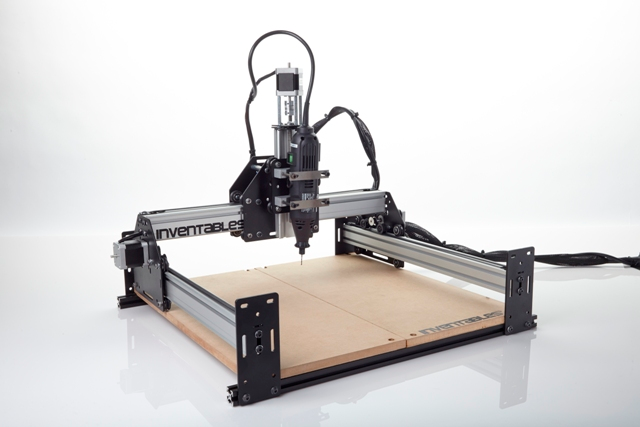
\includegraphics[scale=0.5]{ch-2/image6.png}
	}
	\caption{Трёхкоординатный фрезерный станок, реализованный в рамках открытого проекта \textit{Shapeoko}}\label{fig:shapeoko}
\end{figure}

На данный момент проект находится на очень ранней стадии развития, поэтому не удалось провести детальный и всесторонний анализ недостатков представляемого проекта. Тем не менее, некоторые из них можно выделить уже сейчас:

\begin{itemize}
	\item Проект ориентирован в основном на трёхкоординатную фрезерную обработку и не позиционируется как модульная универсальная платформа.
	\item Управление опять отдаётся на откуп обычного персонального компьютера, за тем лишь исключением, что вместе пакета EMC2 (LinuxCNC) авторы предлагают собственное программное обеспечение. О создании какой-либо модульной электронной системы управления речи не идёт.
	\item Также как и в предыдущем проекте отсутствует какая-либо обратная связь по положению рабочего органа.
	\item Для передвижения портала использованы два шаговых двигателя, никак механически не синхронизированные между собой.
	\item Перемещение портала осуществляется за счёт зубчатых ремней, при этом не предусмотрены датчики обрыва ремня.
	\item Линейное перемещение всех координатных осей осуществляется за счет роликовых кареток. Сложность и~большое количество подвижных частей подобного механизма снижает надежность платформы. Также очевидно, что подобное решение может приводить к заклиниванию осей.
	\item В качестве основного и единственного на сегодняшний день рабочего органа используется гравер.
\end{itemize}

Последний параметр, выбранный для сравнения "--- \textit{модульная открытая архитектура блока управления} в совокупности с открытым исходным микрокодом электронного оборудования.

По данному параметру был найден единственный проект "--- анонсированный на 2015 год корпорацией Google модульный смартфон Ara. Безусловно, трудно производить сравнение модульной системы управления оборудования с ЧПУ и мобильную платформу для создания телефонов и планшетов, но такая цель и не ставилась.

Выбор был обусловлен уникальностью данного проекта. Подобные идеи звучали из уст представителей многих известных компаний и научных центров и ранее, но первая успешная попытка создать достаточно сложное электронное устройство из отдельных взаимозаменяемых модулей была сделана только в этом проекте. Очевидно, что это актуальное направление в ближайшее время получит свое развитие, также очевидно, что оно является очень перспективным и требует всестороннего исследования.

В силу своей специфики достоинства и недостатки проекта Ara рассматриваться не будут, вместо этого будет сделан обзор наиболее интересных и концептуальных решений, реализуемых в рамках данного проекта.

На официальном портале проекта корпорация Google заявляет, что разработала так называемый <<телефон-конструктор>>. Данный конструктор состоит из двух частей: эндоскелета (также часто называемого <<рамой>> и являющегося, по сути, внутренним каркасом) и~набора сменных модулей.

К эндоскелету могут быть подключены процессор со всей необходимой электрической <<обвязкой>>, жидкокристаллический дисплей, дополнительные модули оперативной памяти, физическая клавиатура, камера или дополнительный аккумулятор. Владелец телефон сможет сам производить модернизацию своего устройства или заменять поврежденные модули. Какие-то специальные инструменты или наличие каких-то знаний в области микроэлектроники или программирования не требуются.

Также за счет унификации габаритов эндоскелета и проектируемых модулей можно изменять размер аппарата, предполагается возможность создания как небольшого и очень компактного устройства, так и устройства, сравнимого по своим размерам с современными смартфонами и даже устройства больше похожего на интернет-планшет, а не мобильный телефон.

Очевидное достоинство подобного подхода для пользователя "--- возможность подбирать модули в соответствии со своими потребностями и финансовыми возможностями. Специалисты компании Google говорят, что в минимальной комплектации модульный смартфон будет стоить порядка 50 долларов США, а в максимальной "--- до 500.

Платформа позиционируется как открытая, то есть любой сторонний разработчик, использую так называемый MDK\footnote{сокр.~от~англ. \textit{Module Developers Kit} "--- набор инструментальных средств разработчика для создания модулей.}, сможет выпустить свой модуль, совместимый с Ara.

В спецификации говорится, что некоторые модули могут поддерживать так называемую <<горячую замену>>, то есть возможность сменить модуль без отключения питания аппарата. Также оговорен унифицированный способ крепления модулей к эндоскелету "--- крепление будет осуществляться за счет постоянных магнитов.

Каждый модуль может сочетать в себе несколько различных функций, например, можно создать гибридный модуль, являющийся экраном мобильного телефона и дополнительным аккумулятором, компенсирующим затраты энергии на подсветку и отображение информации.

К сожалению, по состоянию на 2021 год проект Ara в первоначальном состоянии перестал существовать, однако многие наработки, предложенные корпорацией Google, хоть и в несколько упрощенном виде были реализованы в модульном смартфоне Fairphone 3\footnote{Электронный ресурс: {\small\url{fairphone.com}} (дата обращения: 12.12.2019).}.

\section{Современные тенденции в области стандартизации и унификации модульного оборудования}

\subsection{Стандарт МЭК 61499}

Проектирование распределенных систем автоматизации усложняется тем, что не существует единого языка программирования, на котором разработчик мог бы описать всю систему, включая логику каждого узла управления и их взаимодействия. Узлы управления обычно реализуются с использованием программируемых логических контроллеров~(сокр. \textit{ПЛК}), возможно, связанных между собой через различные сети связи. В последнее время в промышленных сетях появилось много других источников и потребителей информации, помимо ПЛК, например, появились интеллектуальные датчики и исполнительные механизмы. В частности, к таким механизмам можно отнести электроприводы или устройства человеко-машинного взаимодействия. Общее поведение таких распределенных систем может быть довольно сложным и иногда чувствительным к незначительным изменениям в поведении каждого участника. Изменения могут быть вызваны не только внутренней логикой, но и различиями в операционных системах, сетевых протоколах, производительности оборудования и т.\,д. До недавнего времени разработчику было сложно реализовать децентрализованную логику распределенного приложения с помощью единого набора инструментальных средств разработки, учитывающего все особенности каждого устройства и их связи, что позволило бы легко отображать и переназначать децентрализованную логику ядра на различные аппаратные архитектуры узлов управления сетью.

Стандарт МЭК 61499 была задумана на перспективу повсеместного использования распределённой автоматизации. Он включает в себя несколько решений основных проблем систем распределенной автоматизации. Можно сказать, что МЭК 61499 предлагает языковой пакет проектирования для распределенных систем измерения и управления, тем самым преодолевая разрыв между популярными языками программирования ПЛК и распределенными системами. Согласно модели МЭК 61499, распределенная система состоит из аппаратных средств, оборудованных интерфейсами с окружающей средой, такими как сети передачи данных или физическое оборудование. Универсальный элемент в архитектуре разработки программного обеспечения в соответствии с МЭК 61499 "--- это функциональный блок.\footnote{От англ. \textit{Functional Block}, сокр. FB.} Функциональные блоки могут использоваться не только для описания логики децентрализованного управления, но также для описания структурных компонентов устройств, таких как их интерфейсы~\cite{patil2018adapting}. Чтобы объединить несколько функциональных блоков в приложение, их соединяют дугами связи событий и данных. Таким образом, полная функциональность распределенной системы управления может быть представлена ​​в терминах функциональных блоков и соединений между ними~\cite{vyatkin2011iec}.

Одной из проблем при разработке систем автоматизации всегда была переносимость программного кодам между программируемыми контроллерами. Необходимость запускать программу на другом типе оборудования возникает часто и по многим причинам. Для решения данной проблемы языки программирования ПЛК были стандартизированы в 1993 году в стандарте IEC 61131-3~\cite{dai2009case}, и теперь все основные поставщики ПЛК заявляют о соответствии своих продуктов этому стандарту. Однако, в отличие от персональных компьютеров, нелегко запустить программу на ПЛК другого производителя. Проблемы могут быть вызваны разным синтаксисом, но во многих случаях они связаны с разной семантикой определенных программных структур.

Еще одна проблема связана с модульными конструкциями. Автоматизированное оборудование часто строится из относительно автономных модулей, каждый со своим алгоритмом управления. Интуитивно удобно организовать управляющий код в соответствии со структурой оборудования~\cite{holm2012iec}. Для этого функции управления отдельными модулями должны быть заключены в программные организационные единицы, которые могут быть собраны в более крупные программы управления целыми комплексами оборудования без изменения их внутренних компонентов. Часто в новом оборудовании повторно используются многие механические компоненты предыдущей модели, как и в программе управления. Более того, это может быть полезно для управления проектированием машины более абстрактным способом, не задумываясь на ранних этапах проектирования о точной аппаратной архитектуре, на которой будет выполняться код. Действительно, во многих случаях аппаратное обеспечение может отличаться, а функциональность и управляющий код могут оставаться (почти) такими же. Например, аппаратное обеспечение может быть одним ПЛК или несколькими ПЛК меньшего размера, подключенными через сеть. Таким образом, распределение программных модулей по конкретным устройствам управления должно быть перенесено на более поздние стадии проектирования. Но было обнаружено, что программные организационные единицы программ PLC не всегда обеспечивают правильную инкапсуляцию, поскольку код, инкапсулированный в таких программных организационных единицах, может вести себя по-разному в зависимости от контекста, в котором он вызывается~\cite{tangermann2004encapsulation}.

Таким образом, переносимость оказалась тесно связанной с инкапсуляцией. Отсутствие переносимости может быть также связано с различиями в синтаксисе или семантике определенных команд языка программирования, но, в более общем плане, из-за разного контекста, в котором вызываются программные модули. Эта проблема уменьшает преимущества модульной конструкции и очень часто встречается при разработке распределенных систем управления.

Архитектура МЭК 61499 предлагает несколько семантических и синтаксических положений для переносимости. Концепция инкапсуляции МЭК 61499 гарантирует защиту внутренних данных функциональных блоков. Блоки можно вызывать только явно, передавая им события. Составные функциональные блоки могут содержать другие экземпляры функциональных блоков, что обеспечивает гибкий механизм модульной конструкции. На синтаксическом уровне существует независимый от производителя формат расширяемого языка разметки для всех универсальных элементов и команд управления устройствами, который позволяет легко обмениваться файлами с устройствами разных производителей ПЛК.

На основании данного стандарта Стамболовым~\cite{stambolov2013development} предложена реконфигурируемая система числового программного управления для модульного фрезерного станка. В качестве аппаратной платформы для проверки полученной модульной системы ЧПУ используются модули UNIMAT, рассматриваемые в разделе~\cref{sec:ch1/industrial-examples}. 

\subsection{Стандрат Module Type Package (MTP)}

На сегодняшний день модульный подход находит свое применение в обрабатывающей промышленности. В частности, наиболее проработанной является концепция NAMUR Module Type Package (MTP), применяемая в областях специальных химических производств, а также в фармацевтической промышленности. Концепция формализована в виде стандарта VDI/VDE/NAMUR 2658~\cite{bernshausen2016namur}. В обрабатывающей промышленности модульные производственные системы играют более важную роль в силу своей повсеместной применимости. Одним из ярких представителей модульного производства в автоматизации производства является стандарт PackML для упаковочных машин. Несмотря на схожие концепции и бизнес-преимущества модульной автоматизации, требования и текущая техническая реализация описания модуля и оркестровки процессов различаются в разных отраслях. Этот факт увеличивает необходимые усилия по внедрению гибридных, то есть межотраслевых приложений. Одним из типичных гибридных приложений является процесс производства химических жидкостей с последующим розливом в бутылки, включая непрерывную часть процесса (например, фактическое производство) и дискретную часть (например, розлив, этикетирование, транспортировку). В работе~\cite{grothoff2020mapping} описывается процесс выявления сходств и различий между существующими подходами к модульной автоматизации. В этом документе основное внимание уделяется интерфейсам управления процессами, которые обычно развертываются в самом модуле и доступны через OPC UA. Наряду с существующими стандартами, такими как MTP и PackML, мы также обсуждаем подход к управлению процессами, который был разработан в рамках финансируемых проектов BaSys 4.0 и BaSys 4.2 и проверен на демонстрации. Для получения инженерной информации о модулях BaSys использует модули, такие как сериализация различных файлов или API (например, интерфейсы XML или RESTful с полезной нагрузкой JSON) или инфраструктуру, подходящую для модульного подхода, например серверы обнаружения для обнаружения компонентов и метаданных.

В соответствии со стандартом MTP производственные модули могут быть от разных производителей, так как функциональность модуля описана в независимой от поставщика оборудования~\cite{bloch2018state}. Одна часть MTP описывает сервисы, которые реализует модуль. В этих сервисах заключены автоматизация полевых устройств модуля и взаимодействие полевых устройств. Таким образом, процесс может быть запущен без необходимости управления отдельными полевыми устройствами. Сервисы являются основным элементом модульных технологических установок, потому что они представляют собой новый уровень в иерархии автоматизации. В дополнении к этому модульная технологическая система содержит человеко-машинный интерфейс блок оркестровки. Блок оркестровки взаимодействует со службами, которые управляют полевыми устройствами в модулях. Прямое влияние на полевые устройства в рабочем автоматическом режиме невозможно, что является самым большим отличием от классических технологических установок. Непрямая адресация полевых устройств с помощью сервисов обеспечивает целостность модуля и защищает ноу-хау поставщика модуля.

Проектирование модульных технологических установок делится на два разных этапа: а) модульное проектирование и б) интеграционное проектирование. На первом этапе поставщик модуля проектирует и реализует модуль, на втором этапе уже в рамках производственного процесса на конкретном предприятии все модули объединяется в единую технологическую установку. Интерфейс между этими двумя "--- это MTP как независимое от производителя описание модуля. На первом этапе проектирования поставщик модуля должен спроектировать сервисы модуля. Следовательно, основные функции процесса в разумных комбинациях должны быть инкапсулированы как сервисы. Следовательно, необходимо учитывать различные аспекты, такие как аспекты проектирования процесса, аспекты устройства и аспекты автоматизации. Поскольку трудно определить, какой способ инкапсуляции и комбинации является разумным, этот вклад сталкивается с инкапсуляцией с точки зрения автоматизации.

\subsection{Концепция Mass Customization}

Концепция массовой персонализации\footnote{От англ. Mass Customization.} также имеет прямое отношение к модульному оборудованию. Как уже отмечалось ранее, в современном производстве наблюдается тенденция к сокращению жизненного цикла выпускаемых изделий и более быстрой смены номенклатуры. Предельным случаем такого направления как раз и является массовая персонализация. В случае массовой персонализации производители не просто сокращают серийность партий одинаковых изделий, но в итоге могут перейти к созданию уникальных вещей, созданных под конкретного потребителя. Это достигается за счёт повышения гибкости производства, когда каждая отдельная единица продукции будет изготавливаться по индивидуальному технологическому процессу, проходя отличные от других схожих с ним изделий этапы производственного цикла. Далее может возникнуть ситуация, когда наличие непрерывно запущенного производства вообще не потребуется. Существенное сокращение технологической подготовки производства позволит выполнять заказы на отдельные виды продукции по мере их поступления. Безусловно, такая гибкость невозможна при использовании классических подходов к технологической подготовке производства и модульное оборудование может стать хорошим подспорьем в этом направлении.

Теоретические основы концепции массовой персонализации были заложены более 40 лет назад. Еще в 1980 году Тоффлер~\cite{toffler1980third} впервые упомянул о ``демассифицированном производстве'' (de-massified production), что говорит о том, что уже в то время некоторые технологии необходимые для персонализации объектов массового производства развились в достаточной степени. В 1993 Пайн~\cite{pine1993mass} впервые описал концепцию Mass Customization, которая получила свое развитие в работе Кота \cite{kotha1995mass}. К 1995 Брауни и~др. описали структуру децентрализованного предприятия, способную поддерживать подобную бизнес-модель~\cite{browne1995future}. Таким образом появились новые направления развития информационной коллаборации в рамках расширенных, а затем и виртуальных предприятий. С появлением концепции Индустрия 4.0 данные направления развития высокотехнологичных производств продолжили совершенствоваться, что в итоге привело к формированию понятий Mass Personalization~\cite{chen2009mass} и HyperAutomation~\cite{park2018fourth}.

Параллельно с развитием концепции Индустрии 4.0 возрастает необходимость совершенствования инструментальных средств цифровизации, в том числе систем поддержки принятия решений (Decision support system). Однако существующие инструменты не достаточно хорошо адаптированы к потенциалу Индустрии 4.0 и не способны удовлетворить быстро изменяющиеся требования клиентов. В статье~\cite{lee2019developing} дается описание процесса создания системы выявления потребностей клиента и преобразование их в требуемые технические характеристики продукта. Для реализации такого подхода используется модель Кано (Kano) и методы оптимизации. Получаемые характеристики передаются в систему поддержки принятия решений верхнего уровня, позволяющую выполнять одновременное проектирование новой конфигурации продукта и изменение производственного цикла. Несмотря на то, что такой подход позволяет успешно учитывать рыночную конъюнктуру на момент запуска продукта, он не позволяет прогнозировать изменения рынка.

Ряд работ посвящен реконфигурации и оптимизация сборочного производства с применением подхода late customization. Россит и~др.~\cite{rossit2019industry} разработали фреймворк для реконфигурации сборочных линий. Данный фреймворк позволяет понять какие изменения необходимо внести в последовательность работы сборочной линии на заключительных этапах производства, чтобы выполнить требования заказчика. Предполагается, что фреймворк должен быть реализован в виде онлайн-системы, предоставляющей клиентам интерактивную систему настройки параметров заказа. Данный подход к анализу требований клиентов позволяет предложить достаточно высокий уровень персонализации готовой продукции, при этом поддерживая уровень производства в соответствии с изменяющейся производственной средой.

Беднар и Рауч~\cite{bednar2019modeling} разработали математическую модель для генерации различных конфигураций выпускаемого продукта на основе комбинации сборочных единиц. Данная модель может быть использована в качестве вспомогательного инструмента для количественной оценки сложности реализации того или иного проекта с точки зрения Mass Customization Production. Модель является автономной и не поддерживает обратной связи с конечным потребителем, а также не учитывает рыночную конъюнктуру.

Также необходимо отметить, что появляются новые подходы, связанные с развитием концепций Mass Customization и Mass Personalization. Например, Ванг и др. \cite{wang2017industry} в своей работе предлагают фреймворк, позволяющий сократить разрыв между Mass Customization и Mass Personalization за счет применения технологий Индустрии 4.0. Предлагается более тесное взаимодействие с конечным потребителем продукции за счет использования усовершенствованной системы заказов, основанной на предпочтениях покупателей. В лабораторных условиях реализована производственная цепочка, демонстрирующая работу Mass Personalization Production, а также представлены примеры практического применения данной концепции в производстве.

Сонг и др.~\cite{song2020product} описывают модель принятия решений для Mass Personalization Production в рамках Индустрии 4.0. В работе приведены теоретические основы и практическая реализация системы сборки высокотехнологичных продуктов с применением принципов стандартизации и избыточности, за счет чего достигается сокращение времени производства и затрат на производственный процесс. В работе~\cite{mourtzis2014web} описывается платформа поддержки принятия решений, ориентированная на Mass Personalization Production. Платформа является адаптивной и позволяет взаимодействовать с клиентами на этапе проектирования продуктов. Предложенное решение интегрировано с платформой децентрализованного производства, реализованной с применением веб-технологий.

Таким образом, можно постулировать, что массовая персонализация является динамично развивающейся концепцией, повсеместно используемой в современном производстве. Гибкость, необходимая для ее реализации достигается различными способами как на уровне планирования, так и на уровне изменения аппаратных средств, используемых в производственном цикле и рассматриваемое в данной работе модульное оборудование может оказать существенное влияние на дальнейшую проработку данной темы.

\section{Выводы по главе 1}

В рамках диссертационной работы исследуются модели и методы построения модульных систем. Подчеркивается, что проблема эффективности работы модульного оборудования до сих пор не решена из-за серьезных различий в подходах к проектированию подобного оборудования и его применения в приборостроительном производстве, что пока не позволяет выполнять эффективное моделирование и переконфигурирования модульных производственных системы. На данный момент не существует эффективных методов и моделей проектирования и разработки модульного оборудования, более того практически отсутствуют единые стандарты проектирования модульного оборудования. Для создания эффективной методики проектирования и использования модульного оборудования необходимо проводить глубокий анализ условий предприятий, работающих в новых и высокоинтеллектуальных отраслях производства, а также в условиях постоянной смены номенклатуры производимых высокотехнологичного оборудования.

\FloatBarrier
